\chapter{Pro-form Gender}
\label{ch:proform-gender}

% Chapter 12: Third Part III case study
% Target: ~6,000 words
% Structure parallels Ch 9 (Countability) and Ch 10 (Definiteness)

\epigraph{\textit{There appears to be a certain amount of learning in losing one's tail; researchers in California found that once a young skink has had a close encounter of the near-fatal kind it seems to be more cautious.}}{— Simon Anderson, \textit{Blink of a Lizard} (2008)}

%--- --- --- --- --- --- --- --- --- --- --- --- --- --- --- --- ---
\section{The puzzle}
\label{sec:12:hook}
%--- --- --- --- --- --- --- --- --- --- --- --- --- --- --- --- ---

Consider two sentences about the same dog:

\ea[]{\label{ex:12:dog-it}\mention{The dog wagged its tail.}}
\z
\ea[]{\label{ex:12:dog-who}\mention{Who's a good boy? Yes, you are!}}
\z
In (\ref{ex:12:dog-it}), the dog takes the non-personal pronoun \mention{it}. In (\ref{ex:12:dog-who}), addressed directly by its owner, the same animal takes the personal pronoun \mention{who} and receives \mention{you}. Nothing about the dog has changed. What changed is how the speaker construed the referent.

This is the puzzle of English gender. Traditional accounts describe a three-way distinction~-- masculine, feminine, neuter~-- realized mainly on pronouns (\mention{he}, \mention{she}, \mention{it}). That description captures something, but it misses the organizing principle. The primary distinction in English gender isn't sex. It's personhood.

The term \term{gender} in linguistics denotes a system of grammatically relevant contrasts wherein certain semantic concepts are divided into a small number of categories. English gender is typically described as referential rather than noun-class: there's no arbitrary assignment to nouns (unlike German \mention{der Tisch}, \mention{die Lampe}), and the choice of pronoun tracks properties of the referent, not grammatical properties of the antecedent \autocite{corbett1991,huddleston2002}. That much is right. But the usual account keeps the scope narrow~-- \mention{he}/\mention{she}/\mention{it}~-- when the system is far wider.

\textcite{siemund2008} models dialectal variation in English pronominal gender as different thresholds on an individuation hierarchy; \textcite{audring2009} shows how pronominal systems resemanticize when agreement is borne primarily by pronouns; \textcite{dolberg2019} traces the transition from lexical to referential gender in the \textit{Anglo-Saxon Chronicle}. These accounts share a common architecture: English gender is referential, hierarchically organized, and driven by properties of the designatum rather than the antecedent. What they also share is a common limitation: they keep the system's scope largely within third-person pronouns.

This chapter shows why that restriction is too narrow. The same personhood-based logic that governs \mention{he}/\mention{she}/\mention{it} also governs \mention{who}/\mention{which}, \mention{somebody}/\mention{something}, and \mention{when}/\mention{where}. The system extends across the entire semantic class of pro-forms~-- items that take their meaning from another element in discourse. This claim requires defense, since these items belong to different lexical categories. I'll address that question after laying out the evidence.

I'll argue that English gender, like countability (Chapter~\ref{ch:countability}) and definiteness (Chapter~\ref{ch:definiteness-and-deitality}), exhibits the HPC architecture: two clusters~-- one semantic (personhood), one lexico-grammatical (the pro-form inventory)~-- coupled by designatum-driven inference and maintained by overlapping mechanisms. Violations aren't just semantic infelicities; they're grammatical errors. The system has teeth.

The puzzle shows up equally clearly in relative pronouns. Consider:


\ea[]{\label{ex:12:doctor-who}\mention{The doctor who I saw was helpful.}}
\z
\ea[]{\label{ex:12:doctor-which}\ungram{\mention{The doctor which I saw was helpful.}}}
\z
\ea[]{\label{ex:12:book-which}\mention{The book which I read was helpful.}}
\z
\ea[]{\label{ex:12:book-who}\ungram{\mention{The book who I read was helpful.}}}
\z

The constraint is robust in standard written English. \mention{Who} for persons, \mention{which} for non-persons (I mean the fused-head use, where \mention{which} stands alone as a relative; non-fused \mention{which}, as in \mention{which person}, is unrestricted). The violations in (\ref{ex:12:doctor-which}) and (\ref{ex:12:book-who}) aren't merely odd~-- they're ungrammatical, comparable to agreement errors or subcategorization violations. This isn't pragmatic markedness; it's grammar.\footnote{Some constraints in the system are categorical in standard written English (\mention{who}/\mention{which}; core \mention{he}/\mention{she}/\mention{it} uses); others show the graded edge behaviour typical of HPC kinds (compound determinatives under shifted construals; chain-coherence effects). Where I mark examples with an asterisk, the notation indicates failure under the intended construal, not string ill-formedness.}

The same split appears in interrogatives:

\ea[]{\label{ex:12:int-who}\mention{Who's coming to the party?} \hfill [asking about persons]}
\z
\ea[]{\label{ex:12:int-what}\mention{What's in your purse?} \hfill [asking about non-persons]}
\z
\ea[]{\label{ex:12:int-who-bad}\ungram{\mention{Who's in your purse?}} \hfill [under construal: asking about objects]}
\z
\ea[]{\label{ex:12:int-what-bad}\ungram{\mention{What's coming to the party?}} \hfill [under construal: asking about persons]}
\z
Examples (\ref{ex:12:int-who-bad}) and (\ref{ex:12:int-what-bad}) are grammatical only under shifted construals~-- if the speaker expects a person in the purse or a non-person attending the party. The choice of interrogative reveals the speaker's conceptualization of the potential referent.

This is the \mention{who}/\mention{which} puzzle. Relative pronouns are not usually discussed under the heading of ``gender,''\footnote{Both \textcite{huddleston2002} and \textcite{quirk1985} treat the personal/non-personal distinction as a separate axis from the \mention{he}/\mention{she}/\mention{it} sex-based contrast. Most grammars fail to recognize the 
distinction at all.} but their distribution obeys exactly the same personhood-based constraint that governs \mention{he}/\mention{she}/\mention{it}. The puzzle dissolves when we recognize that both are manifestations of a single hierarchical system.

%--- --- --- --- --- --- --- --- --- --- --- --- --- --- --- --- ---
\section{The hierarchy}
\label{sec:12:hierarchy}
%--- --- --- --- --- --- --- --- --- --- --- --- --- --- --- --- ---

The English pro-form gender system is hierarchically organized. At the top level, the distinction is between \term{personal} and \term{non-personal}. Within personal, there's a further split between \term{epicene} (unmarked for sex) and \term{sexual} (masculine/feminine). Within non-personal, productive subtypes include \term{locative} and \term{temporal}.

\begin{figure}[htbp]
\centering
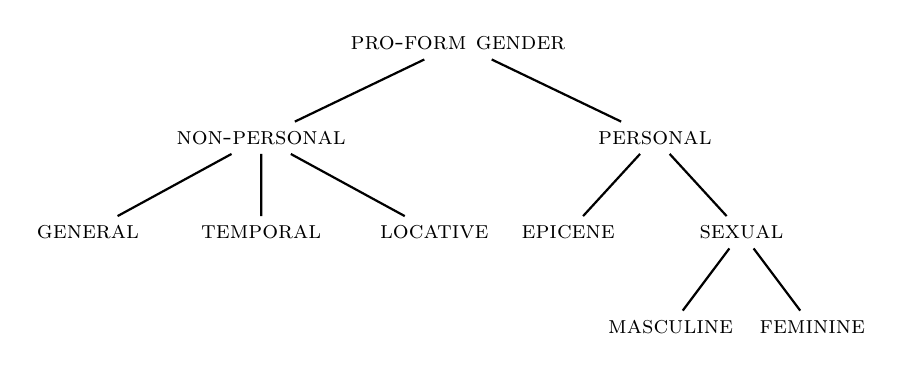
\begin{tikzpicture}[
  level distance=1.2cm,
  sibling distance=3.5cm,
  every node/.style={font=\small\scshape},
  edge from parent/.style={draw, thick},
  level 1/.style={sibling distance=5cm},
  level 2/.style={sibling distance=2.2cm},
  level 3/.style={sibling distance=1.8cm}
]
\node {pro-form gender}
  child {node {non-personal}
    child {node {general}}
    child {node {temporal}}
    child {node {locative}}
  }
  child {node {personal}
    child {node {epicene}}
    child {node {sexual}
      child {node {masculine}}
      child {node {feminine}}
    }
  };
\end{tikzpicture}
\caption{Hierarchy of gender values for English pro-forms.}
\label{fig:12:hierarchy}
\end{figure}

Each subtype inherits the properties of its parent. A word with feminine gender is necessarily sexual, which is necessarily personal. A word with locative gender is necessarily non-personal.

Table~\ref{tab:12:inventory} shows the inventory. The leftmost column lists gender-neutral pro-forms~-- items that impose no presuppositional constraint on the designatum. The remaining columns list gender-sensitive items, distinguished by the personhood constraint they encode.

\begin{table}[htbp]
\caption{The pro-form gender system of English.}
\label{tab:12:inventory}
\small
\setlength{\tabcolsep}{4pt}
\centering
\begin{tabular}{@{}p{2.2cm}p{2.0cm}p{1.5cm}p{1.5cm}p{2.5cm}p{1.0cm}p{1.0cm}@{}}
\toprule
\multicolumn{1}{c}{Gender-neutral} & \multicolumn{6}{c}{Gender-sensitive} \\
\cmidrule(l){1-1} \cmidrule(l){2-7}
& \multicolumn{3}{c}{Non-personal} & \multicolumn{3}{c}{Personal} \\
\cmidrule(lr){2-4} \cmidrule(l){5-7}
& General & Temporal & Locative & Epicene & \multicolumn{2}{c}{Sexual} \\
\cmidrule(l){2-2} \cmidrule(l){3-3} \cmidrule(l){4-4} \cmidrule(l){5-5} \cmidrule(l){6-7}
& & & & & Masc & Fem \\
\midrule
\mention{they}\textsubscript{pl} & \mention{it} & \mention{then} & \mention{there} & \mention{I}, \mention{we}\textsubscript{pron}, \mention{you}\textsubscript{pron}, \mention{they}\textsubscript{sg}, \mention{one}\textsubscript{gen} & \mention{he} & \mention{she} \\
\addlinespace
\mention{whose}\textsubscript{rel} & \mention{what}, \mention{which} & \mention{when} & \mention{where} & \mention{who}, \mention{whom}, \mention{whose}\textsubscript{int} \\
\addlinespace
\mention{this}, \mention{that} & & & \mention{here} & \mention{we}\textsubscript{det}, \mention{you}\textsubscript{det} \\
\addlinespace
& \mention{-thing} & & \mention{-where} & \mention{-body}, \mention{-one} \\
\bottomrule
\end{tabular}
\par\smallskip\noindent\footnotesize\textit{Note.} Subscripts: \textsubscript{pl}~=~plural; \textsubscript{sg}~=~singular; \textsubscript{gen}~=~generic; \textsubscript{rel}~=~relative; \textsubscript{int}~=~interrogative; \textsubscript{pron}~=~pronoun; \textsubscript{det}~=~determinative (as in \mention{we linguists}, \mention{you guys}).
\end{table}

Several entries require comment. Plural \mention{they} is gender-neutral: it can refer to persons (\mention{There are some people. They are tall}) or non-persons (\mention{There are some trees. They are tall}) without constraint. Singular \mention{they}, however, is personal: \mention{There's a person. They are tall} is grammatical, but \mention{*There's a tree. They are tall} is not \autocite{bjorkman2017,konnellycowper2020}. The difference is that singular \mention{they} presupposes a personal designatum; plural \mention{they} does not.

Similarly, relative \mention{whose} is compatible with both personal and non-personal antecedents (\mention{the person/book whose story is well known}), while interrogative \mention{whose} normally carries a personal presupposition (\mention{Whose coat is this?}). The split reflects how these items function: relative \mention{whose} inherits its construal from the antecedent; interrogative \mention{whose} presupposes personhood independently.

I include first- and second-person pronouns (\mention{I}, \mention{we}, \mention{you}) to show the inventory's personhood partition. These are epicene personal: they can only refer to entities construed as persons (using \mention{I} for an inanimate object requires personification), but they don't encode sexual gender. Nothing in the analysis turns on sex marking for these items.

The table reveals a system far larger than the traditional \mention{he}/\mention{she}/\mention{it} triad. The compound determinatives~-- \mention{somebody}/\mention{something}, \mention{everyone}/\mention{everything}, \mention{anywhere}/\mention{anyone}~-- participate in the same personhood partition. The relative pro-forms \mention{where} and \mention{when} encode non-personal subtypes parallel to \mention{which}.

%--- --- --- --- --- --- --- --- --- --- --- --- --- --- --- --- ---
\section{Designatum-driven gender}
\label{sec:12:designatum}
%--- --- --- --- --- --- --- --- --- --- --- --- --- --- --- --- ---

Before examining the mechanism, a clarification. The English system tracks the \term{designatum}~-- the entity as conceptualized by the speaker~-- not the referent (the real-world correlate) or the antecedent (the linguistic controller). The \term{designatum} is what a linguistic term designates; the \term{referent} is ``some independently distinguishable entity, or set of entities, in the real world'' \autocite[399]{huddleston2002}. The \term{antecedent} is the ``constituent whose meaning dictates the meaning of a pronoun or other such expression in cases of anaphora'' \autocite[295]{huddleston2005}.

This distinction is crucial. A pro-form need not have an antecedent to participate in the gender system: interrogative \mention{who} designates a person even though it has neither referent nor antecedent. The designatum need not be a token: \mention{the typical politician is not to be trusted} designates a type, but the gender is still personal. And the designatum can diverge from the antecedent's lexical properties.

The English system differs from antecedent-driven systems in exactly this way. In Spanish, French, or German, gender assignment is fixed on nouns and agreement spreads through NP-internal morphology. The antecedent controls the pro-form.

In English, it's the designatum~-- how the referent is conceptualized~-- that controls selection. The source provides the constraint; the pro-form satisfies it.

Consider a case of referential metonymy:

\ea[]{\label{ex:12:metonymy}\mention{The French fries is waiting. She's upset.} \hfill \autocite{wu2025}}
\z
An NP with a default non-personal reading (\mention{the French fries}) is used to invoke a customer; subsequent anaphora tracks that metonymic designatum, yielding personal-feminine \mention{she}. The antecedent's form (plural, non-personal) doesn't control the pro-form; the conceptualized source does.

Spanish does not readily permit this kind of pro-form shift while retaining ordinary agreement with the same antecedent NP. (The English number mismatch~-- plural label, singular verb~-- reflects a menu-item construal orthogonal to the pro-form point; in Spanish I keep agreement normal to isolate the controller issue.)

\ea\label{ex:12:spanish}
    \ea[{*}]{\gll \mention{Las} \mention{patatas} \mention{fritas} \mention{esperan}. \mention{Él} \mention{está} \mention{enfadado}.\\
    \textsc{def.f.pl} potato.\textsc{f.pl} fried.\textsc{f.pl} wait.\textsc{3pl.pres} \textsc{3sg.m} be.\textsc{3sg.pres} angry.\textsc{m.sg}\\
    \glt Intended: `The French fries are waiting. He's upset.'}
    \ex[]{\gll \mention{Las} \mention{patatas} \mention{fritas} \mention{esperan}. \mention{El} \mention{señor} \mention{está} \mention{enfadado}.\\
    \textsc{def.f.pl} potato.\textsc{f.pl} fried.\textsc{f.pl} wait.\textsc{3pl.pres} \textsc{def.m.sg} gentleman.\textsc{m.sg} be.\textsc{3sg.pres} angry.\textsc{m.sg}\\
    \glt `The French fries are waiting. The gentleman is upset.'}
    \z
\z
Spanish requires grammatical agreement with the antecedent (\textit{patatas}, feminine plural), not semantic agreement with the metonymic designatum. The speaker typically recasts the controller with a human-denoting NP like \mention{\textit{el señor}} (`the gentleman') to achieve the intended reference. English permits categorical shifts based on conceptualization because it lacks NP-internal gender agreement: the designatum-driven pathway is freer. This is the signature of a designatum-driven system.


%--- --- --- --- --- --- --- --- --- --- --- --- --- --- --- --- ---
\section{The inventory}
\label{sec:12:inventory}
%--- --- --- --- --- --- --- --- --- --- --- --- --- --- --- --- ---

Standard accounts keep gender within personal pronouns. \textcite[486]{huddleston2002} state that English gender is ``based purely on pronoun agreement.'' But the evidence shows the system extends across all pro-forms~-- the semantic class of items that take their meaning from another element in discourse.

What unifies pro-forms is their interpretive dependence: they have minimal 
descriptive content and take their value from context~-- linguistic, 
situational, or conceptual. A pronoun \enquote{stands for} an NP; a pro-adverb \enquote{stands for} an adverb phrase; a \mention{wh}-word \enquote{stands for} a constituent in a question or relative clause. This isn't a morphosyntactic category (there's no frame that selects for ``any pro-form''), but a semantic one. The gender constraint doesn't respect lexical-category boundaries: whatever property licenses \mention{who} also licenses \mention{somebody} and blocks \mention{something}.

Recall the skink in the epigraph: first \mention{one's} (epicene personal, attributing the capacity to learn), then \mention{it} (non-personal, the default for a lizard). The chain shifts from personal to non-personal across clauses~-- exactly the kind of construal shift that §\ref{sec:12:chain-coherence} will show is possible but marked.

\subsection{Determinatives}
\label{sec:12:determinatives}

The compound determinatives with \mention{-body} and \mention{-one} are personal:

\ea[]{\label{ex:12:somebody}\mention{Somebody left their coat.} \hfill [personal]}
\z
\ea[]{\label{ex:12:somebody-bad}\ungram{\mention{Somebody is in your purse.}} \hfill [under construal: referring to an object]}
\z
Example (\ref{ex:12:somebody-bad}) is ungrammatical unless \mention{somebody} refers to a person who is in the purse. These are epicene~-- they don't encode sex~-- but they do encode the personal/non-personal distinction.

The compound determinatives with \mention{-thing} and \mention{-where} are non-personal:

\ea[]{\label{ex:12:something}\mention{Something is on the table.} \hfill [non-personal]}
\z
\ea[]{\label{ex:12:something-bad}\ungram{\mention{Everything enjoyed themselves.}} \hfill [under construal: personal referents]}
\z
Example (\ref{ex:12:something-bad}) requires personification to be grammatical. The boundary is discourse-driven rather than syntactically hard~-- exactly the HPC-style graded edge we expect.

\subsection{Relative pro-forms}
\label{sec:12:relative-proforms}

The distinction between \mention{where}/\mention{when} and \mention{which} parallels the distinction between \mention{who} and \mention{which}:

\ea[]{\label{ex:12:room-where}\mention{the room where the painting was done} \hfill [room as location]}
\z
\ea[]{\label{ex:12:room-which}\mention{the room which was painted} \hfill [room as patient]}
\z

\ea[]{\label{ex:12:2010-when}\mention{2010, when I left} \hfill [as time]}
\z
\ea[]{\label{ex:12:2010-which}\mention{2010, which has 365 days} \hfill [as entity]}
\z
The same source (\mention{room}, \mention{2010}) takes different pro-forms depending on how it's conceptualized. This is designatum-driven selection applied to locative and temporal subtypes.


%--- --- --- --- --- --- --- --- --- --- --- --- --- --- --- --- ---
\section{How the system holds together}
\label{sec:12:coupling}
%--- --- --- --- --- --- --- --- --- --- --- --- --- --- --- --- ---

\subsection{Chain coherence}
\label{sec:12:chain-coherence}

Once a designatum is construed as personal or non-personal within a reference chain, mixing is disfavoured. Consider:

\ea[]{\label{ex:12:dog-chain-a}\mention{That's the dog who attacked his owner.} \hfill [personal chain]}
\z
\ea[]{\label{ex:12:dog-chain-b}\mention{That's the dog which attacked its owner.} \hfill [non-personal chain]}
\z
\ea[{}]{\label{ex:12:dog-chain-c}\mmark{\mention{That's the dog which attacked his owner.}} \hfill [mixed]}
\z
\ea[{}]{\label{ex:12:dog-chain-d}\mmark{\mention{That's the dog who attacked its owner.}} \hfill [mixed]}
\z
Examples (\ref{ex:12:dog-chain-a}) and (\ref{ex:12:dog-chain-b}) are fully acceptable~-- coherent personal and non-personal chains. Examples (\ref{ex:12:dog-chain-c}) and (\ref{ex:12:dog-chain-d}) are degraded~-- the chain starts in one gender and shifts to another mid-sentence.

This is \term{chain-internal coherence}. The constraint isn't absolute~-- discourse can independently reclassify a designatum (personification, stance shift)~-- but absent such cues, speakers prefer consistency within a reference chain. The contrast is strongest when the speaker is not deliberately shifting stance.

Chain coherence is a maintenance mechanism. It stabilizes the personhood assignment across discourse, reinforcing the clustering of pro-forms around a shared construal.

\subsection{The coupling}
\label{sec:12:coupling-subsec}

We now have the architecture. On the semantic side sits the \term{personhood cluster}: the conceptual properties that make a referent construable as a person~-- intentionality, agency, consciousness, reciprocal treatment. These cluster because personhood is a natural cognitive category, grounded in Theory of Mind and social cognition \autocite{waytz2010}. \textcite{dennett1976} lists conditions for personhood (rationality, consciousness, reciprocal treatment, self-awareness); I use these illustratively, not as necessary conditions that speakers compute. What matters is that person-attribution is cognitively basic and socially consequential.

On the lexico-grammatical side sits the \term{pro-form inventory}: the gender-sensitive lexical items and their distributional constraints~-- the personal pronouns (\mention{he}/\mention{she}/\mention{it}/\mention{they}), the pro-nominal \mention{one}, \mention{who}/\mention{which} in relative clauses, \mention{-body}/\mention{-thing} in compound determinatives, and designated slots for personal and non-personal reference. (Pro-form is a semantic grouping; what I'm tracking here is its \emph{realization}~-- the specific forms and where they're licensed.)

The two clusters are coupled by \term{designatum-driven inference}. When speakers produce a pro-form, they signal how they're construing the referent. When hearers process a pro-form, they infer the construal. The inference runs bidirectionally: form cues construal; construal constrains form.

This parallels the bidirectional inference that couples individuation to count morphosyntax (Chapter~\ref{ch:countability}) and identifiability to deitality (Chapter~\ref{ch:definiteness-and-deitality}). The coupling is what produces the HPC signature: properties that statistically co-occur, maintained by causal mechanisms, with graded membership at the edges.

\subsection{The machinery of maintenance}
\label{sec:12:maintenance}

In Chapter~\ref{ch:stabilizers}, we surveyed the general machinery that maintains linguistic kinds. For pro-form gender, three mechanisms seem to do the heaviest work.

\term{Cognitive grounding} provides the anchor. Personhood attribution is cognitively basic~-- grounded in Theory of Mind, face processing, and social cognition \autocite{waytz2010,carey2009}. Infants distinguish agents from non-agents within months of birth; by 12 months they attribute goals to entities that act contingently \autocite{csibra2003}. The person/non-person boundary is among the earliest conceptual distinctions humans make. This gives the personhood cluster a stability that categories like Old English masculine, feminine, and neuter lack: it's rooted in pre-linguistic cognition, not just in distributional patterns.

\term{Semantic transparency} reinforces the coupling. The mapping from personhood to pro-form is largely predictable: if you know a referent is construed as a person, you can predict the pro-form inventory it will take. This transparency makes the system easy to learn and stable under transmission. Compare countability, where object-mass nouns like \mention{furniture} create opaque exceptions, or definiteness, where weak definites break the form--meaning correspondence. Gender has fewer such mismatches: the \mention{who}/\mention{which} alternation tracks personhood with high fidelity. The transparency of the mapping may facilitate acquisition: children do not produce the systematic gender-agreement errors characteristic of grammatical-gender languages when learning the \mention{who}/\mention{which} distinction, though direct acquisition studies of this specific contrast remain sparse.

\term{error and repair} operates through chain coherence and social charge. If a speaker were to shift from \mention{who} to \mention{it} mid-chain, hearers would notice. The mismatch would trigger puzzlement, clarification requests, or mental correction. Crucially, gender mismatches are socially charged in a way that many grammatical errors aren't: calling a person \mention{it} is an insult; misgendering someone with \mention{he} when \mention{she} is appropriate triggers conversational repair \autocite{mcconnell-ginet2014}. This repair pressure keeps the personal/non-personal boundary sharp even as individual items (pets, robots) shift position on the personhood spectrum.

These three mechanisms~-- cognitive grounding, semantic transparency, error and repair~-- seem best positioned to explain the system's distinctive stability. Standard mechanisms (acquisition, entrenchment, transmission) also apply, but they don't explain why gender is more stable than, say, the count/non-count distinction for \mention{data}. The stability likely emerges from the convergence: personhood is cognitively basic, the mapping is transparent, and violations are repaired.


%--- --- --- --- --- --- --- --- --- --- --- --- --- --- --- --- ---
\section{Evidence and limits}
\label{sec:12:evidence}
%--- --- --- --- --- --- --- --- --- --- --- --- --- --- --- --- ---

\subsection{Cross-linguistic scope}
\label{sec:12:cross-linguistic}

Is pro-form gender an English peculiarity or a cross-linguistic pattern?

The personhood distinction appears remarkably widespread. \textcite{haspelmath1997} notes that ``the distinction between human and non-human referents is made practically everywhere (`who' vs.\ `what', `somebody' vs.\ `something'), even in languages where humanness isn't very prominent elsewhere in the grammar'' (34--35). Languages with rich antecedent-driven gender (Spanish \mention{quién}/\mention{qué}, German \mention{wer}/\mention{was}, French \mention{qui}/\mention{quoi}) still make the personhood split in their interrogative and indefinite systems. The personhood partition may be cognitively more basic than the particular morphosyntactic systems that realize it.

What's distinctive about English isn't the personhood distinction itself but its \term{scope}. Because English lacks NP-internal gender agreement, the designatum-driven pathway is unconstrained by formal concord. Speakers can shift a referent's construal without generating agreement violations. The \mention{who}/\mention{which} alternation, the \mention{-body}/\mention{-thing} compounds, and the chain-coherence effects are all more prominent in English precisely because they're not overridden by noun-class agreement.

Dialectal variation within English shows the system's parameters. \textcite{siemund2008} documents varieties (Southwest England, Newfoundland, Tasmania) where the personal/non-personal cut shifts: \mention{he} and \mention{she} extend to inanimates based on a mass/count distinction rather than personhood. The hierarchy's structure remains stable; its semantic basis varies. This suggests the architecture is robust but its semantic grounding is a parameter that communities can tune.

\subsection{Passing the tests}
\label{sec:12:tests}

Chapter~\ref{ch:failure-modes} introduced the Two-Diagnostic Test for genuine HPC kinds: high projectibility and robust homeostasis.

Knowing a pro-form's gender predicts its distribution. If you know \mention{somebody} is personal, you can predict it will combine with personal predicates, take personal reflexives (\mention{themselves}), and resist non-personal contexts. If you know \mention{which} is non-personal, you can predict it cannot take human antecedents without personification.

Crucially, knowing the designatum's construal predicts pro-form selection. If you know the speaker is construing a pet as personal, you can predict \mention{who} over \mention{which}, \mention{he}/\mention{she} over \mention{it}. The predictions are bidirectional: from form to construal, from construal to form.

The clustering is maintained by mechanisms. Acquisition transmits the system as a unit; entrenchment preserves high-frequency patterns; alignment provides real-time stabilization; transmission filters for learnability. Perturb any mechanism~-- expose children to non-standard input, isolate speakers from conversational feedback~-- and the cluster should degrade. But it doesn't scatter randomly; the degradation should track the mechanisms involved.

The clustering isn't just a statistical regularity. It's causally maintained.

\subsection{Where the clusters slip}
\label{sec:12:slippage}

Like countability and definiteness, the pro-form gender system shows characteristic slippage. These aren't anomalies; they're evidence of the underlying dual-cluster architecture.

\subsection{Pets and anthropomorphism}
\label{sec:12:pets}

Pets occupy the boundary. \textcite{shirvertesh2012} demonstrates that pets are often treated as persons, but flexibly~-- the attribution can shift with situation. This flexibility appears in pronoun usage:

\ea[]{\label{ex:12:cat-it}\mention{The cat licked its paw.} \hfill [non-personal default]}
\z
\ea[]{\label{ex:12:cat-she}\mention{Poor Whiskers! She's not feeling well.} \hfill [personified]}
\z
Same referent, different construals. The slippage is systematic: speakers shift between personal and non-personal based on discourse framing, emotional involvement, and naming.

\subsection{Collectives}
\label{sec:12:collectives}

Collective nouns present a related puzzle:

\ea[]{\label{ex:12:team-its}\mention{The team has scored its first goal.} \hfill [singular, non-personal]}
\z
\ea[]{\label{ex:12:team-their}\mention{The team have scored their first goal.} \hfill [plural, personal]}
\z
The variation tracks construal: team-as-entity versus team-as-members. But combining singular verb with plural personal anaphora is marked:

\ea[]{\label{ex:12:team-themself}\mmark{\mention{The team has scored on themselves.}}}
\z
Many speakers accept singular verb + plural anaphora with collectives (\mention{The team has changed their strategy}), so the constraint is not absolute. What is stable is the preference: the combination of singular verb with singular personal reflexive (\mention{*The team has scored on themself}) is strongly disfavoured. Collectives expose a tension between individuation and personhood: singular construals resist person-marking unless the construal shifts to plural.

\subsection{Infants}
\label{sec:12:infants}

Human infants, paradigmatic persons, can take non-personal \mention{it}:

\ea[]{\label{ex:12:baby-it}\mention{The baby was crying because it was hungry.}}
\z
This isn't a denial of personhood; it reflects temporary withholding of person-status~-- often when sex is unknown or when the discourse foregrounds non-personal properties \autocite{mcconnell-ginet2014}. The slippage reveals that personhood is an attribution, not a biological fact.

\subsection{The \mentionhead{which}/\mentionhead{what}/\mentionhead{something} asymmetry}
\label{sec:12:asymmetry}

Not all non-personal items behave identically. \textcite[499]{huddleston2002} note that \mention{which} can serve as an antecedent to \mention{he} or \mention{she}:

\ea[{}]{\label{ex:12:which-he}\mmark{\mention{That's the dog which attacked his owner.}}}
\z
This parallels the mid-sentence number shift we find with collectives. But the same shift seems degraded with \mention{what} and \mention{something}:

\ea[{}]{\label{ex:12:what-he}\mmmark{\mention{What attacked his owner was this dog.}}}
\z
\ea[{*}]{\label{ex:12:something-he}\mention{Something attacked his owner.} \hfill [with coreference]}
\z
If these judgments are robust, \mention{something} and \mention{what} pattern with \mention{it} in resisting personal anaphora, while \mention{which} is more permissive. This might reflect gradience within the non-personal domain: some items are prototypically non-personal (\mention{something}, \mention{it}), others more marginal (\mention{which}). The asymmetry deserves systematic investigation.


%--- --- --- --- --- --- --- --- --- --- --- --- --- --- --- --- ---
\section{Looking forward}
\label{sec:12:transition}
%--- --- --- --- --- --- --- --- --- --- --- --- --- --- --- --- ---

Pro-form gender is a localized system. The relevant constraints are carried by a specific semantic class of lexical items~-- those that function as pro-forms~-- and enforced across anaphoric chains. The coupling between personhood and morphosyntax is tight within that domain.

The final case study pushes to the widest scope. Lexical categories like \term{noun} and \term{verb} look strikingly stable cross-linguistically, while \term{adjective} and \term{adposition} vary dramatically. If these are HPC kinds, the mechanisms that maintain them must be far more diffuse~-- operating across the entire grammar, not just within a circumscribed inventory. Chapter~\ref{ch:lexical-categories} asks what happens when the coupling is weak, the mechanisms are partial, and the cluster boundaries are contested.
